\documentclass[11pt]{article}

% ------
% LAYOUT
% ------
\textwidth 165mm %
\textheight 230mm %
\oddsidemargin 0mm %
\evensidemargin 0mm %
\topmargin -15mm %
\parindent= 10mm

\usepackage[dvips]{graphicx}
\usepackage{multirow,multicol}
\usepackage[table]{xcolor}

\usepackage{amssymb}
\usepackage{amsfonts}
\usepackage{amsthm}
\usepackage{amsmath}

\usepackage{subfigure}
\usepackage{minted}

\graphicspath{{./pix/}} % put all your figures here.

\begin{document}
\begin{center}
\Large{\textbf{ECE 595: Homework 2}}

Yi Qiao, Class ID 187

(Spring 2019)
\end{center}

\section*{Exercise 1}
\subsection*{(a)}
Refer to code in the back. 
\subsection*{(b)}
The data was successfully read, shown by the screen below.
\begin{figure}[h]
	\centering
	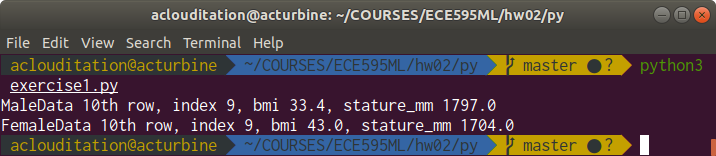
\includegraphics[width=0.7\linewidth]{exercise1.png}
	\caption{screenshot for reading data}
\end{figure}

\section*{Exercise 2}
\subsection*{(a)}
\begin{equation}	\label{eq2(a)}
\begin{split}
\begin{bmatrix}\pmb{\omega}^*\\ \omega^*_0\end{bmatrix}
&=\underset{\pmb{\omega},\omega_0}{argmin}\sum_{j=1}^N(\pmb{\omega}^T\pmb{x}_j+\omega_0-y_j)^2\\
set\ \pmb{\theta}&=\begin{bmatrix}\pmb{\omega}^*\\ \omega^*_0\end{bmatrix}\\
\pmb{\theta}^*&=\underset{\pmb{\theta}}{argmin}\sum_{j=1}^N(\begin{bmatrix}\pmb{x}_j^T & 1\end{bmatrix}\pmb{\theta}-y_j)^2\\
\end{split}
\end{equation}
\begin{center}
thus,\\
$$A=\begin{bmatrix}
-\pmb{x}_1- & 1\\
-\pmb{x}_2- & 1\\
...& ...\\
-\pmb{x}_N- & 1\\
\end{bmatrix}\ 
\pmb{b}=\begin{bmatrix}
y_1\\
y_2\\
...\\
y_N
\end{bmatrix}$$
\end{center}
\subsection*{(b)}
by least square
\begin{equation}	\label{eq2(b)}
\begin{split}
\pmb{A}^T\pmb{A\theta}^*&=\pmb{A}^T\pmb{b}\\
\pmb{\theta}^*&=(\pmb{A}^T\pmb{A})^{-1}\pmb{A}^T\pmb{b}
\end{split}
\end{equation}
if $A^TA$ is invertible, $A$ needs to be full column rank (or $null(A)=0$).
TODO: find out how to avoid this issue

\subsection*{(c)}
Refer to the code in the back.\\
The optimal weight $\theta^*$ is:\\
$$\pmb{\theta}^* = \begin{bmatrix}
-1.23396767e-2\\
6.67486843e-3\\
-1.07017505e+1
\end{bmatrix}$$

\subsection*{(d)}
Refer to the code in the back again.\\
The weight vector computed using CVXPY is the same as
the one computed in the previous step.\\
$$\pmb{\theta}^* = \begin{bmatrix}
-1.23396767e-2\\
6.67486843e-3\\
-1.07017505e+1
\end{bmatrix}$$
\section*{Exercise 3}

\subsection*{(a)}
\subsubsection*{(i)}
\begin{figure}[h]
	\centering
	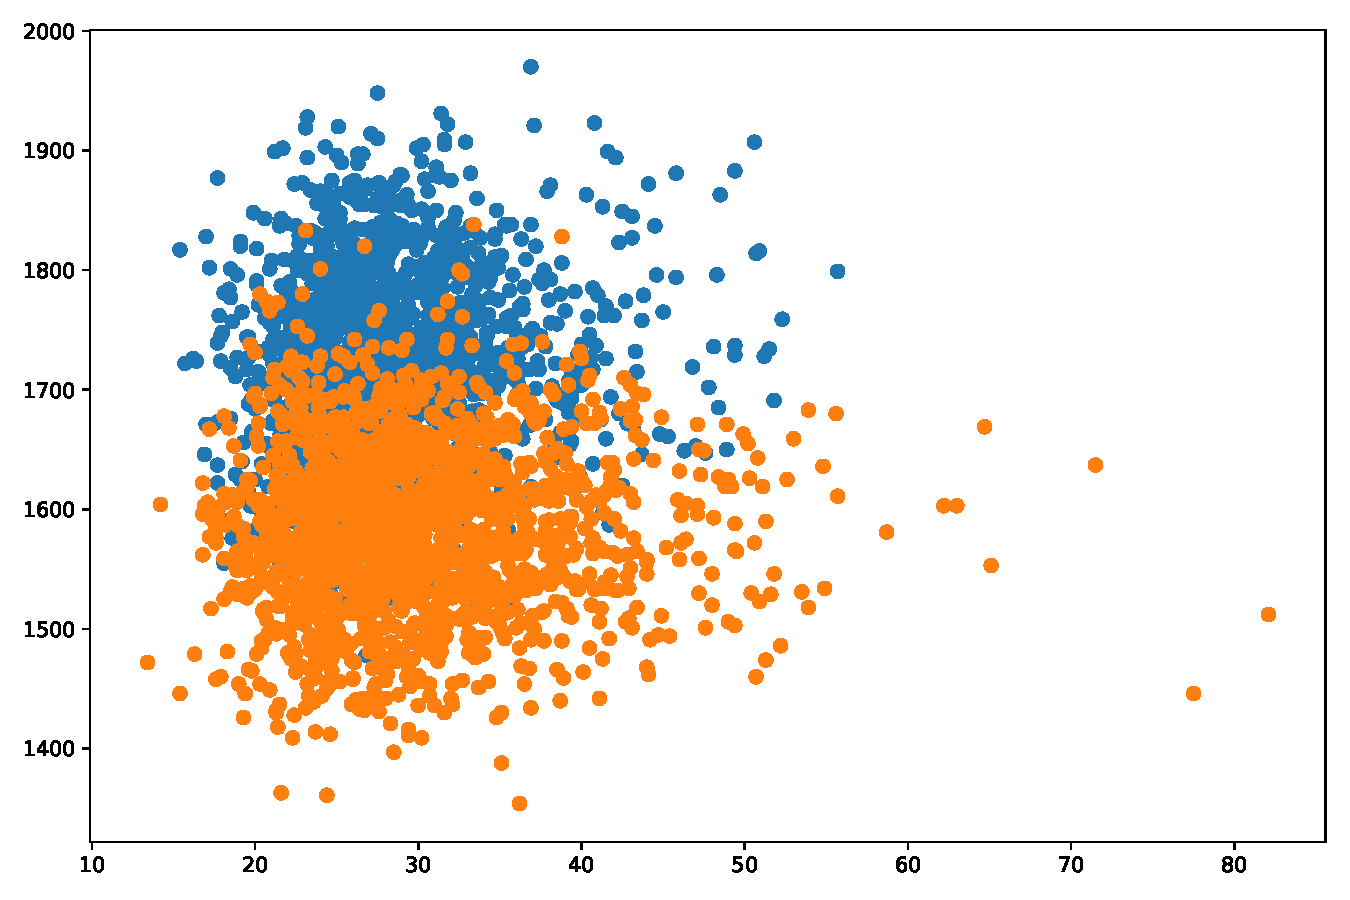
\includegraphics[width=0.5\linewidth]{exercise3_1}
	\caption{Training data}
\end{figure}
\subsubsection*{(ii)}

\begin{equation}
\begin{split}
\pmb{\omega}^{*T}\pmb{x}+\omega_0^*&=0\\
\omega_1^*x_1+\omega_2^*x_2+\omega_0^*&=0\\
x_2=-\frac{\omega_1^*x_1+\omega_0^*}{\omega_2^*}
\end{split}
\end{equation}
\subsubsection*{(iii)}
\begin{figure}[h]
	\centering
	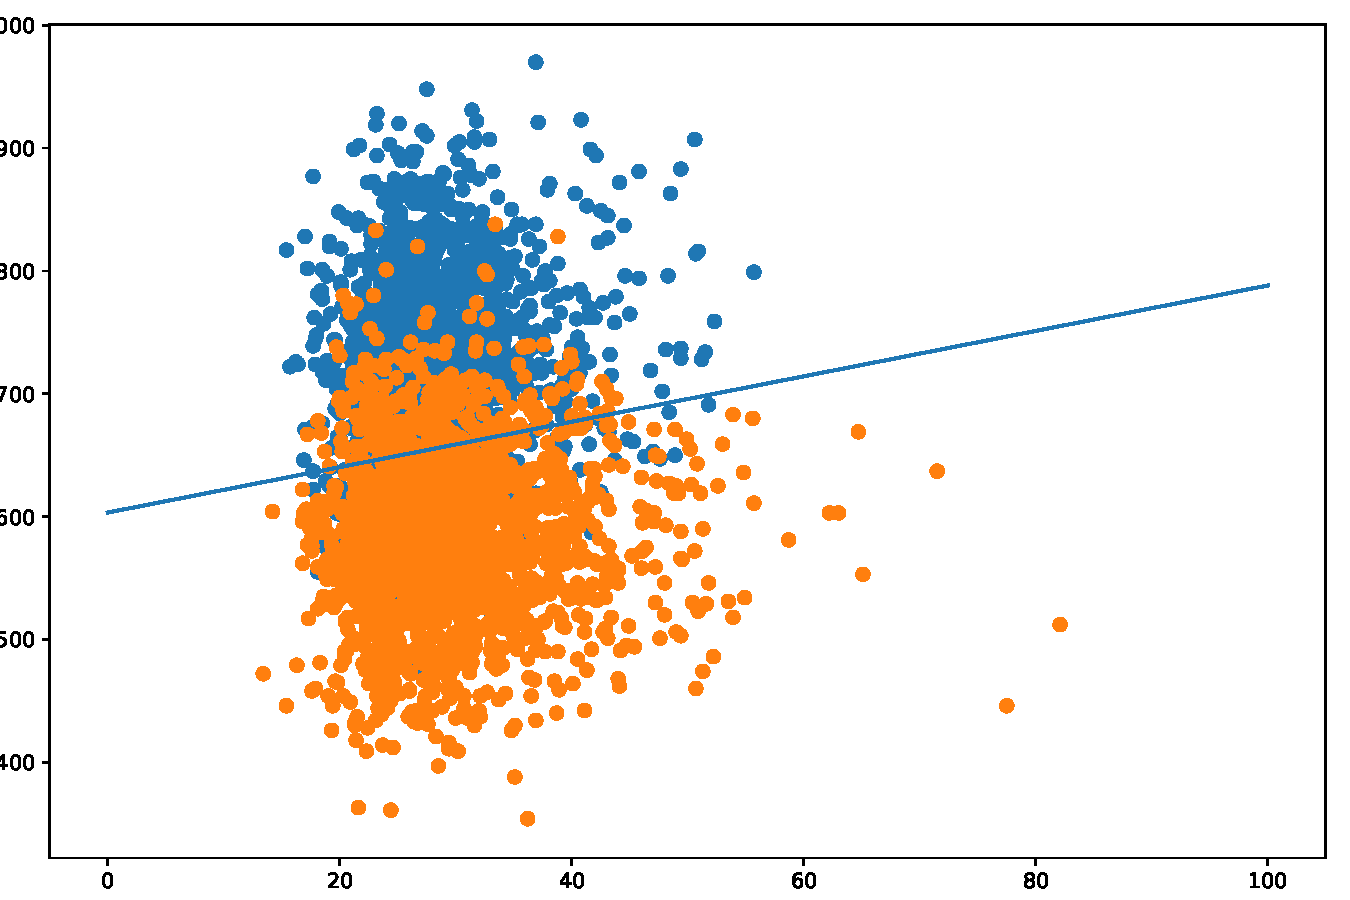
\includegraphics[width=0.5\linewidth]{exercise3_2}
	\caption{Training data with decision boundary}
\end{figure}
\subsection*{(b)}
Refer to the code in the back, the success rate is:
$$success\ rate = 83.93\%$$
\pagebreak
\section*{Exercise 4}
\subsection*{(a)}
\subsubsection*{(i)}
\begin{figure}[h]
	\centering
	\subfigure[1]{
		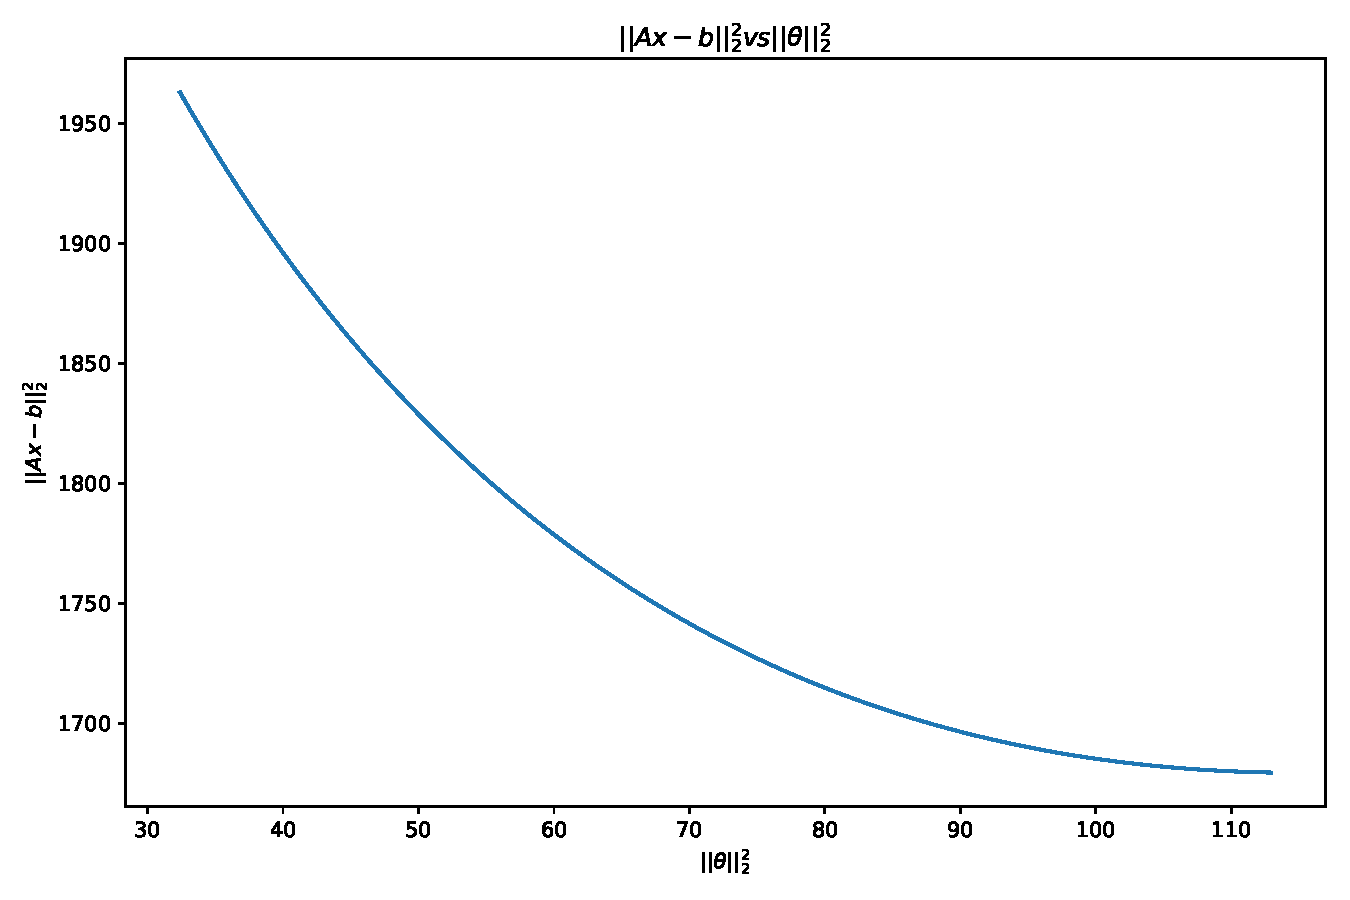
\includegraphics[width=0.47\linewidth]{exercise4_1}
	}
	\subfigure[2]{
		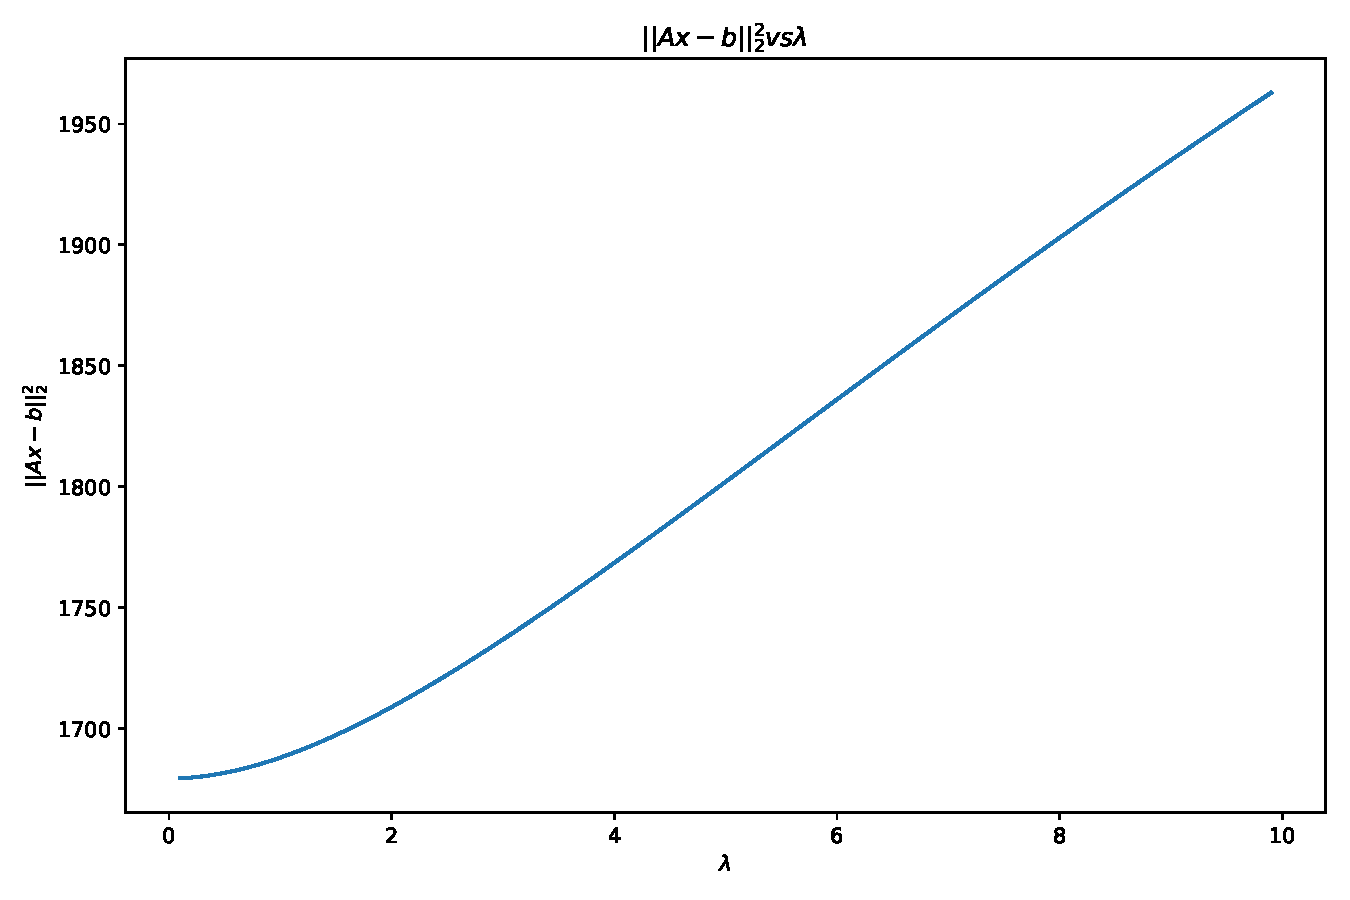
\includegraphics[width=0.47\linewidth]{exercise4_2}	
	}
	\subfigure[3]{
		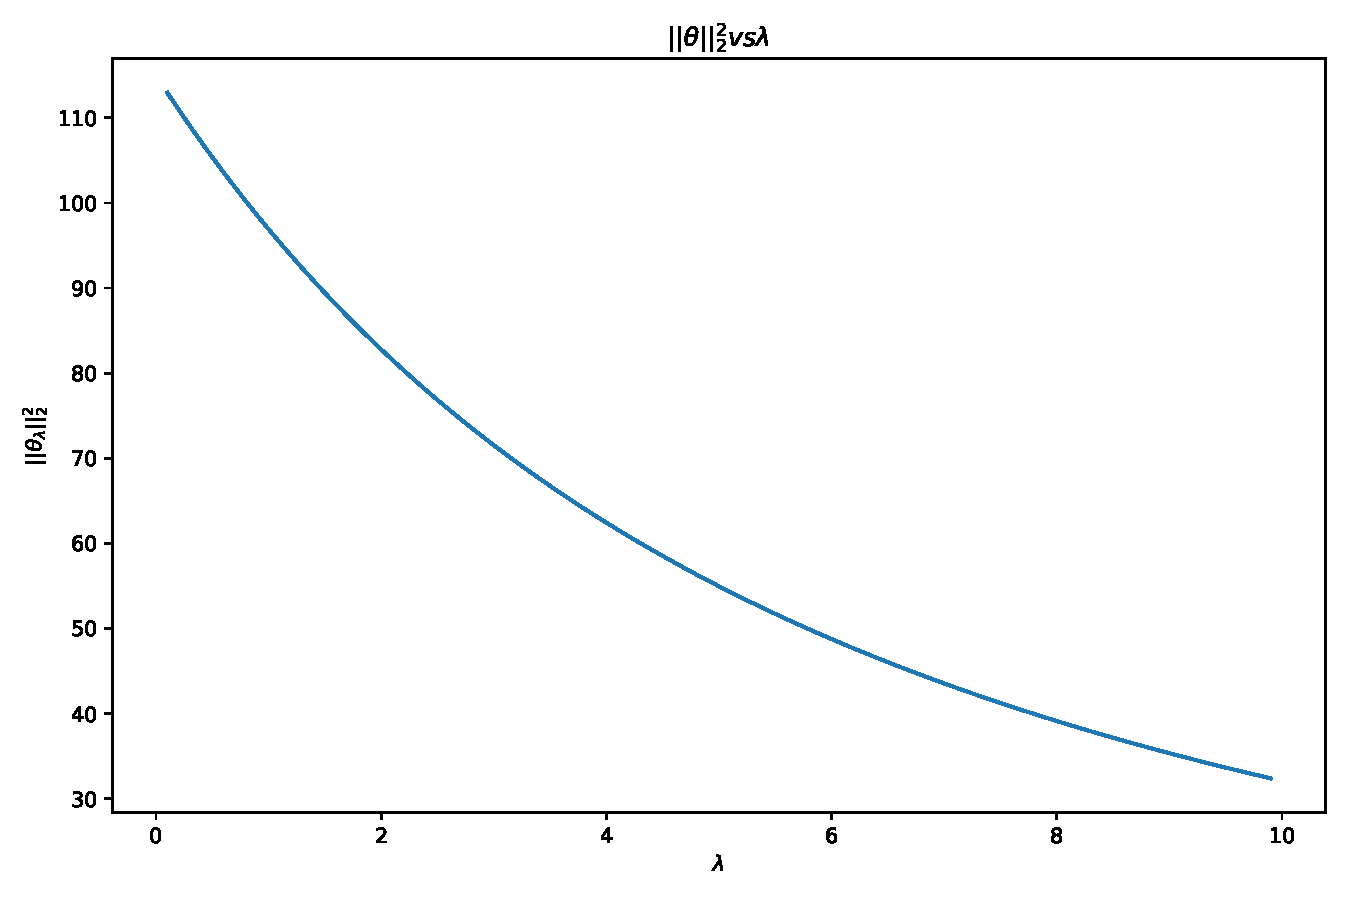
\includegraphics[width=0.47\linewidth]{exercise4_3}	
	}	
	\subfigure[4]{
		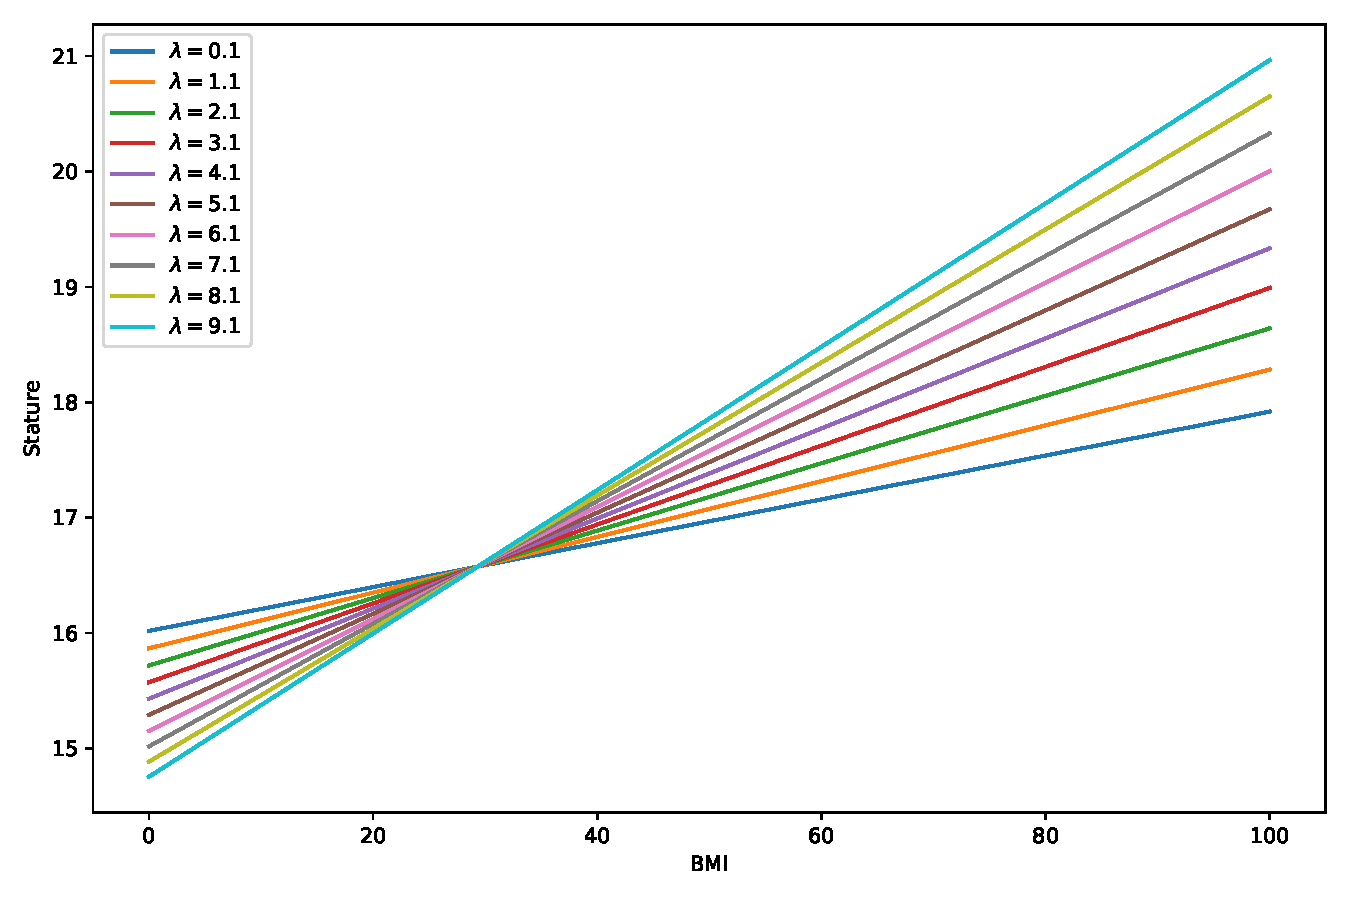
\includegraphics[width=0.47\linewidth]{exercise4}
	}
\end{figure}
\subsubsection*{(ii)}
TODO: fix this
\subsection*{(b)}
\subsubsection*{(i)}
for equation (8), $\pmb{\theta}_\lambda=\underset{\pmb{\theta}}{argmin}||\pmb{A\theta}-\pmb{b}||^2_2+\lambda||\pmb{\theta}||^2_2$:\\
\begin{equation}
\mathcal{L}(\pmb{\theta})=||\pmb{A\theta}-\pmb{b}||^2_2+\lambda||\pmb{\theta}||^2_2
\end{equation}
Since no constraint, the vertex can be found at:
\begin{equation}
\begin{split}
\nabla_\theta||\pmb{A\theta}-\pmb{b}||^2_2+\lambda\nabla_\theta||\pmb{\theta}||^2_2&=0\\
2\pmb{A}^T(\pmb{A\theta}-\pmb{b})+2\lambda\pmb{\theta}&=0\\
\pmb{A}^T\pmb{A\theta}+\lambda\pmb{\theta}&=\pmb{A}^T\pmb{b}\\
\pmb{\theta}_\lambda=(\pmb{A}^T\pmb{A}+\lambda\pmb{I})^{-1}\pmb{A}^T\pmb{b}
\end{split}
\end{equation}
for equation (9), $\pmb{\theta}_\alpha=\underset{\pmb{\theta}}{argmin}||\pmb{A\theta}-\pmb{b}||^2_2 \ subject\ to\ ||\pmb{\theta}||^2_2\le\alpha$, $\alpha-||\pmb{\theta}||^2_2\ge 0$ :
\begin{equation}
\mathcal{L}(\pmb{\theta},\gamma)=||\pmb{A\theta}-\pmb{b}||^2_2-\gamma(\alpha-||\pmb{\theta}||^2_2)
\end{equation}
KKT conditions:\\
\begin{equation}
\begin{aligned}
\nabla_\theta||\pmb{A\theta}-\pmb{b}||^2_2+\gamma\nabla_\theta(||\pmb{\theta}||^2_2-\alpha)&=0 &\ stationarity\\
\alpha-||\pmb{\theta}||^2_2&\ge 0 &\ primal\ feasibility\\
\gamma&\ge 0 &\ dual\ feasibility\\
\gamma(\alpha-||\pmb{\theta}||^2_2)&=0 &\ complementary\ slackness
\end{aligned}
\end{equation}
for equation (10),
$\pmb{\theta}_\epsilon=\underset{\pmb{\theta}}{argmin}||\pmb{\theta}||^2_2\ subject\ to\ ||\pmb{A\theta}-\pmb{b}||^2_2\le\epsilon$, $\epsilon-||\pmb{A\theta}-\pmb{b}||^2_2\ge 0$:
\begin{equation}
\mathcal{L}(\pmb{\theta},\gamma)=||\pmb{\theta}||^2_2-\gamma(\epsilon-||\pmb{A\theta}-\pmb{b}||^2_2)
\end{equation}
KKT conditions:\\
\begin{equation}
\begin{aligned}
\nabla_\theta||\pmb{\theta}||^2_2+\gamma\nabla_\theta(||\pmb{A\theta}-\pmb{b}||^2_2-\epsilon)&=0 &\ stationarity\\
\epsilon-||\pmb{A\theta}-\pmb{b}||^2_2&\ge 0 &\ primal\ feasibility\\
\gamma&\ge 0 &\ dual\ feasibility\\
\gamma(\epsilon-||\pmb{A\theta}-\pmb{b}||^2_2)&=0 &\ complementary\ slackness
\end{aligned}
\end{equation}

\subsubsection*{(ii)}
for equation (9), stationarity suggests that:
\begin{equation}
\nabla_\theta||\pmb{A\theta}-\pmb{b}||^2_2+\gamma\nabla_\theta(||\pmb{\theta}||^2_2-\alpha)=0
\end{equation}
by doing the algebra, we get:
\begin{equation}
\begin{split}
2\pmb{A}^T(\pmb{A\theta}-\pmb{b})+2\gamma\pmb{\theta}=0\\
\pmb{\theta}_\alpha=(\pmb{A}^T\pmb{A}+\gamma\pmb{I})^{-1}\pmb{A}^T\pmb{b}
\end{split}
\end{equation}
if we set $\gamma_\alpha=\lambda$, referring to equation (5) above:\\
\begin{equation}
\begin{split}
\pmb{\theta}_\alpha&=(\pmb{A}^T\pmb{A}+\lambda\pmb{I})^{-1}\pmb{A}^T\pmb{b}\\
&=\pmb{\theta}_\lambda
\end{split}
\end{equation}
where primal feasibility:
$$\alpha-||\pmb{\theta}_\alpha||^2_2\ge 0$$
is satisfied if we choose $\alpha = ||\pmb{\theta}_\lambda||^2_2$ since $\pmb{\theta}_\alpha = \pmb{\theta}_\lambda$,\\
	$$\alpha-||\pmb{\theta}_\alpha||^2_2=||\pmb{\theta}_\alpha||^2_2-||\pmb{\theta}_\alpha||^2_2=0\ge0$$
Dual feasibility is automatically satisfied since we fix $\gamma_\alpha=\lambda>0$\\
Complementary slackness is satisfied since 	$\alpha-||\pmb{\theta}_\alpha||^2_2=0$\\

\noindent Thus, the two problems (8) and (9) are equivalent.
\subsubsection*{(iii)}
for equation (9), stationarity suggests that:
\begin{equation}
\nabla_\theta||\pmb{\theta}||^2_2+\gamma\nabla_\theta(||\pmb{A\theta}-\pmb{b}||^2_2-\epsilon)=0
\end{equation}
by doing the algebra, we get:
\begin{equation}
\begin{split}
2\pmb{\theta}+2\gamma\pmb{A}^T(\pmb{A\theta}-\pmb{b})&=0\\
\pmb{\theta}_\epsilon&=(\gamma\pmb{A}^T\pmb{A}+\pmb{I})^{-1}\pmb{A}^T\gamma\pmb{b}\\
\pmb{\theta}_\epsilon&=(\gamma^{-1}\gamma\pmb{A}^T\pmb{A}+\gamma^{-1}\pmb{I})^{-1}\pmb{A}^T\pmb{b}\\
\pmb{\theta}_\epsilon&=(\pmb{A}^T\pmb{A}+\gamma^{-1}\pmb{I})^{-1}\pmb{A}^T\pmb{b}
\end{split}
\end{equation}
if we set $\gamma_\epsilon=\lambda^{-1}$, referring to equation (5) above:\\
\begin{equation}
\begin{split}
\pmb{\theta}_\epsilon&=(\pmb{A}^T\pmb{A}+\lambda\pmb{I})^{-1}\pmb{A}^T\pmb{b}\\
&=\pmb{\theta}_\lambda
\end{split}
\end{equation}
where primal feasibility:
$$\epsilon-||\pmb{A\theta}_\epsilon-\pmb{b}||^2_2\ge 0$$
is satisfied if we choose $\epsilon = ||\pmb{A\theta}_\lambda-\pmb{b}||^2_2$ since $\pmb{\theta}_\epsilon = \pmb{\theta}_\lambda$,\\
$$\epsilon-||\pmb{A\theta}_\epsilon-\pmb{b}||^2_2=0\ge0$$
Dual feasibility is automatically satisfied since we fix $\gamma_\epsilon^{-1}=\lambda>0$, thus, $
\gamma_\epsilon > 0$\\
Complementary slackness is satisfied since 	$\epsilon-||\pmb{A\theta}_\epsilon-\pmb{b}||^2_2=0$\\

\noindent Thus, the two problems (8) and (10) are also equivalent.
\pagebreak
\subsection*{(c)}
\subsubsection*{(i)}
\begin{figure}[h]
	\centering
	\subfigure[1]{
		\includegraphics[width=0.47\linewidth]{exercise4_4}
	}
	\subfigure[2]{
		\includegraphics[width=0.47\linewidth]{exercise4_5}	
	}
	\subfigure[3]{
		\includegraphics[width=0.47\linewidth]{exercise4_6}	
	}	
\end{figure}
\subsubsection*{(ii)}
\begin{figure}[h]
	\centering
	\subfigure[1]{
		\includegraphics[width=0.47\linewidth]{exercise4_7}
	}
	\subfigure[2]{
		\includegraphics[width=0.47\linewidth]{exercise4_8}	
	}
	\subfigure[3]{
		\includegraphics[width=0.47\linewidth]{exercise4_9}	
	}	
\end{figure}
\subsection*{(d)}
\end{document}

